\documentclass[10pt]{beamer}
\usetheme[
%%% options passed to the outer theme
%    progressstyle=movCircCnt,   %either fixedCircCnt, movCircCnt, or corner
%    rotationcw,          % change the rotation direction from counter-clockwise to clockwise
%    shownavsym          % show the navigation symbols
  ]{AAUsimple}
  
% If you want to change the colors of the various elements in the theme, edit and uncomment the following lines
% Change the bar and sidebar colors:
%\setbeamercolor{AAUsimple}{fg=red!20,bg=red}
%\setbeamercolor{sidebar}{bg=red!20}
% Change the color of the structural elements:
%\setbeamercolor{structure}{fg=red}
% Change the frame title text color:
%\setbeamercolor{frametitle}{fg=blue}
% Change the normal text color background:
%\setbeamercolor{normal text}{fg=black,bg=gray!10}
% ... and you can of course change a lot more - see the beamer user manual.
  \usepackage{multimedia}
\usepackage[utf8]{inputenc}
\usepackage[english]{babel}
\usepackage[T1]{fontenc}
% Or whatever. Note that the encoding and the font should match. If T1
% does not look nice, try deleting the line with the fontenc.
\usepackage{helvet}
\usepackage{comment}
\usepackage{standalone}
\usepackage{longtable}
\usepackage{pbox}
\usepackage[table]{xcolor}
\definecolor{light-gray}{gray}{0.8}
%\rowcolors{1}{magenta}{cyan}
%\rowcolors{1}{}{light-gray}
\let\oldtabular\tabular
\let\endoldtabular\endtabular
\renewenvironment{tabular}{\global\rownum=0\relax\oldtabular}{\endoldtabular}
\usepackage[acronym,toc,nomain]{glossaries}
\makeglossaries
\usepackage{etex}
\usepackage{makecell}
\usepackage{bytefield}
\usepackage{xcolor,colortbl}
\usepackage{a4wide}
\usepackage[inner=1.5in, outer=1.0in, bottom=1in]{geometry}
\usepackage[utf8] {inputenc}
\usepackage[T1] {fontenc}
% \usepackage{amsmath}
\usepackage{amsthm} % is included in mathtools
\newtheorem{theorem}{Theorem}
\usepackage{mathtools}
\usepackage{relsize}
\usepackage{hhline}
\DeclarePairedDelimiter{\ceil}{\lceil}{\rceil}
\DeclarePairedDelimiter{\floor}{\lfloor}{\rfloor}
\usepackage{amsfonts}
\usepackage{verbatim}
\usepackage{todonotes}
\usepackage{calc}
\usepackage{algorithm}
\usepackage{algorithmicx}
\makeatletter
\renewcommand{\ALG@beginalgorithmic}{\scriptsize}
\makeatother
\usepackage{algpseudocode}
\usepackage{multirow}
\usepackage{array}
\usepackage{styles/arydshln}
\usepackage{styles/pgf-umlsd}
\usepackage{pgfgantt}
\algtext*{EndWhile}% Remove "end while" text
\algtext*{EndIf}% Remove "end if" text
\algtext*{EndFor}% Remove "end for" text
\usepackage{caption}
\usepackage{subcaption}
\usepackage{setspace}
\usepackage{pdfpages}
\usepackage{booktabs}
\usepackage{enumitem}
\setitemize{noitemsep}
\usepackage{wrapfig}
\usepackage{pgfplots}
\usepackage{tikz}
\usetikzlibrary{chains}
\usepgflibrary{shapes.geometric}
\usetikzlibrary{shapes}
\usetikzlibrary{calc}
\usetikzlibrary{arrows}
\usetikzlibrary{automata}
\usetikzlibrary{patterns}
\usetikzlibrary{positioning}
\usepackage{styles/tikz-3dplot}
\usepackage{ifthen}
\usepackage{xifthen}
\usepackage{xstring}
\usepackage{pgfopts}
\usepackage{calc}
\usepackage{rotating}
\usepackage{styles/tikz-uml}
\tikzset{
  labelC node/.style={
    at end,align=center,above=-0.08cm,xshift=-6,sloped,
    font=\footnotesize,
    execute at begin node=\setlength{\baselineskip}{0.7em},
    node distance=5cm        
%     append after command={%    
%     \pgfextra
%       \node[draw,near end]{#1};
%       \node[labelB node,middle]{#2}
%       \node[draw,near start]{#3} 
% %      \node[at end, above right]{#2};     
% %      \node[at end, above right]{#3};
%     \endpgfextra
%     }
  },
  labelD node/.style={    
    at start,align=center,sloped,right=-0.08cm,xshift=6,
    rotate=-90,
    font=\footnotesize,
    execute at begin node=\setlength{\baselineskip}{0.7em},
    node distance=5cm        
  }
}
\newcommand{\conceptionalclassbox}[2]{%
\begin{tikzpicture}
\draw (0,0)  node[rectangle,minimum height=0.7cm,draw,minimum width=2.1cm,align=center](satellite){};
\draw (satellite) node[align=center,font=\scriptsize] {#1};
\draw (satellite) node[minimum height=1cm,minimum width=2.1cm,draw,below of=satellite,align=left,font=\scriptsize,node distance =0.85cm](diagram){};
\draw (diagram.north west) node[anchor=north west,align=left,font=\scriptsize] {#2};
\end{tikzpicture}
}
\tikzset{>=stealth',shorten >=1pt,
  object node/.style={
    circle,align=center,
    minimum size=2cm,inner sep=0pt,
    draw
    % font=\sffamily\normalsize\bfseries
  },
  control node/.style={
    circle,dashed,align=center,
    minimum size=2cm,inner sep=0pt,
    draw
    % font=\sffamily\Large\bfseries
  },
  labelA node/.style={
    midway,align=center,above=-0.08cm,sloped,
    font=\footnotesize,
    execute at begin node=\setlength{\baselineskip}{0.7em},
    node distance=5cm
  },
  labelB node/.style={
    midway,align=center,below=-0.08cm,sloped,
    font=\footnotesize,
    execute at begin node=\setlength{\baselineskip}{0.7em},
    node distance=5cm
  },
  labelKrillo node/.style={
    midway,align=center,right=-0.08cm,yshift=2,
    font=\footnotesize,
    execute at begin node=\setlength{\baselineskip}{0.7em},
    node distance=5cm
  },
  labelInvKrillo node/.style={
    midway,align=center,left=-0.08cm,yshift=2,
    font=\footnotesize,
    execute at begin node=\setlength{\baselineskip}{0.7em},
    node distance=5cm
  },
  data node/.style={
    align=center,
    execute at begin node=\setlength{\baselineskip}{1em},
    append after command={%
      \pgfextra
      \draw [-]  (\tikzlastnode.south east) to (\tikzlastnode.south west);
      \draw [-]  (\tikzlastnode.north east) to (\tikzlastnode.north west);
      \endpgfextra
    }
  },
  terminate node/.style={
    align=center,
    execute at begin node=\setlength{\baselineskip}{0.7em}
  },
  task node/.style={
    trapezium,
    trapezium left angle=50,
    trapezium right angle=-50,
    align=center,
    minimum height=1cm, minimum width=4cm, draw,
    append after command={%
    \pgfextra
        \node[draw=none,fill=none, align=center] at (\tikzlastnode.center) {#1};
    \endpgfextra
    }
  },
  harry_potter1 node/.style={
    align=center,minimum height=1.5cm,
    minimum width=0.5cm, rotate=25, anchor = south,
    append after command={%
    \pgfextra
        \node[draw=none,fill=none, align=center] at ([xshift=10, yshift=7]\tikzlastnode.north) (1) {#1};
        \draw  plot [tension=1] coordinates {(\tikzlastnode.north east) ([xshift=5, yshift=-5]\tikzlastnode.center) ([xshift=-5, yshift=5]\tikzlastnode.center) (\tikzlastnode.south west)};
    \endpgfextra
    }
  },
  harry_potter2 node/.style={
    align=center,minimum height=1.5cm,
    minimum width=0.5cm, rotate=25, anchor = south,
    append after command={%
    \pgfextra
        \node[draw=none,fill=none, align=center] at ([xshift=-5, yshift=-10]\tikzlastnode.south) (1) {#1};
        \draw  plot [tension=1] coordinates {(\tikzlastnode.south west) ([xshift=-5, yshift=5]\tikzlastnode.center) ([xshift=5, yshift=-5]\tikzlastnode.center) (\tikzlastnode.north east)};
    \endpgfextra
    }
  },
  queue_v node/.style n args={3}{
    align=center,midway,anchor=center,
    rotate around={#2:(0,0)},
    minimum height = 10, minimum width = 15,
    append after command={%
    \pgfextra
        \draw node[draw=none, fill=white, anchor=south west, rotate=#2, minimum height = 10, minimum width = 15,] at (\tikzlastnode.south west) {};
        \draw node[anchor=north, rotate=90, align=center, font=\footnotesize,
  execute at begin node=\setlength{\baselineskip}{0.9em}] at ([xshift=10]\tikzlastnode.center) {\footnotesize #1};
          \draw[-] plot coordinates {([yshift=#3*4]\tikzlastnode.north west) (\tikzlastnode.south west) (\tikzlastnode.south east) ([yshift=#3*5]\tikzlastnode.north east)};
          \draw[-] plot coordinates {(\tikzlastnode.north east) (\tikzlastnode.north west) (\tikzlastnode.west) (\tikzlastnode.east) (\tikzlastnode.south east)};
    \endpgfextra
    }
  },
  queue_h node/.style n args={3}{
    align=center,midway,anchor=center,
    rotate around={#2:(0,0)},
    minimum height = 15, minimum width = 10,
    append after command={%
    \pgfextra
        \draw node[draw=none, fill=white, anchor=south west, rotate=#2, minimum height = 15, minimum width = 10] at (\tikzlastnode.south west) {};
        \draw node[anchor=south, rotate=0, align=center, font=\footnotesize,execute at begin node=\setlength{\baselineskip}{0.9em}] at ([yshift=8]\tikzlastnode.center) {#1};
          \draw[-] plot coordinates {([xshift=-#3*4]\tikzlastnode.south west) (\tikzlastnode.south east) (\tikzlastnode.north east) ([xshift=-#3*5]\tikzlastnode.north west)};
          \draw[-] plot coordinates {(\tikzlastnode.north west) (\tikzlastnode.south west) (\tikzlastnode.south) (\tikzlastnode.north) (\tikzlastnode.north west)};
    \endpgfextra
    }
  },
  loose_v node/.style n args={3}{
    align=center,midway,anchor=center,
    rotate around={#2:(0,0)},
    minimum height = 10, minimum width = 15,
    append after command={%
    \pgfextra
        \draw node[draw=none, anchor=south west, rotate=#2, minimum height = 10, minimum width = 15,] at (\tikzlastnode.south west) {};
        \draw node[anchor=north, rotate=90, align=center, font=\footnotesize,execute at begin node=\setlength{\baselineskip}{0.9em}] at ([xshift=10]\tikzlastnode.center) {\footnotesize #1};
        \draw[-] plot coordinates {([yshift=#3*4]\tikzlastnode.north west) (\tikzlastnode.south west) (\tikzlastnode.south east) ([yshift=#3*5]\tikzlastnode.north east)};
    \endpgfextra
    }
  },
  loose_h node/.style n args={3}{
    align=center,midway,anchor=center,
    rotate around={#2:(0,0)},
    minimum height = 15, minimum width = 10,
    append after command={%
    \pgfextra
        \draw node[draw=none, anchor=south west, rotate=#2, minimum height = 15, minimum width = 10] at (\tikzlastnode.south west) {};
        \draw node[anchor=south, rotate=0, align=center, font=\footnotesize,execute at begin node=\setlength{\baselineskip}{0.9em}] at ([yshift=8]\tikzlastnode.center) {#1};
          \draw[-] plot coordinates {([xshift=-#3*4]\tikzlastnode.south west) (\tikzlastnode.south east) (\tikzlastnode.north east) ([xshift=-#3*5]\tikzlastnode.north west)};
    \endpgfextra
    }
  },
  reply_h node/.style n args={4}{
    align=center,midway,anchor=center,
    rotate around={#3:(0,0)},
    minimum height = 15, minimum width = 15,
    append after command={%
    \pgfextra
        \draw node[anchor=center, rotate=0, align=center, font=\footnotesize,execute at begin node=\setlength{\baselineskip}{0.9em}] at ([yshift=(#4*16)+#4*16]\tikzlastnode.center) {\footnotesize #1};
        \draw node[anchor=center, rotate=0, align=center, font=\footnotesize,execute at begin node=\setlength{\baselineskip}{0.9em}] at ([yshift=-#4*22]\tikzlastnode.center) {\footnotesize #2};
        \draw[-] plot coordinates {(\tikzlastnode.south east) (\tikzlastnode.south west) (\tikzlastnode.north west) (\tikzlastnode.north east) ([yshift=#4*15]\tikzlastnode.north east) ([yshift=#4*15,xshift=-#4*16]\tikzlastnode.north east)};
    \endpgfextra
    }
  },
  reply_v node/.style n args={4}{
    align=center,midway,anchor=center,
    rotate around={#3:(0,0)},
    minimum height = 15, minimum width = 15,
    append after command={%
    \pgfextra
        \draw node[anchor=west, rotate=0, align=center, font=\footnotesize,execute at begin node=\setlength{\baselineskip}{0.9em}] at ([xshift=(1+#4)*-24+(1-#4)*8]\tikzlastnode.west) {\footnotesize #1};
        \draw node[anchor=east, rotate=0, align=center, font=\footnotesize, execute at begin node=\setlength{\baselineskip}{0.9em}] at ([xshift=(1+#4)*15]\tikzlastnode.east) {\footnotesize #2};
        \draw[-] plot coordinates {(\tikzlastnode.north east) (\tikzlastnode.south east) (\tikzlastnode.south west) (\tikzlastnode.north west) ([xshift=-#4*15]\tikzlastnode.north west) ([xshift=-#4*15,yshift=-#4*16]\tikzlastnode.north west)};
    \endpgfextra
    }
  },
  data node/.style={
    rectangle,align=center,
    minimum width=2cm,minimum height=1.cm,
    inner sep=0pt,
    draw
   },
   start node/.style={
     circle,fill=black,align=center,
     minimum size=0.75cm,inner sep=0pt,draw
  },
  end node/.style={
     circle, align=center, minimum size=0.75cm, draw,
     append after command = {
     \pgfextra
        \draw node[circle, align=center, minimum size = 0.5cm, fill=black] at (\tikzlastnode.center) {};
     \endpgfextra
     }
  },
  single_queue_v node/.style n args={3}{
    align=center,midway,anchor=center,
    rotate around={#2:(0,0)},
    minimum height = 10, minimum width = 15,
    append after command={%
    \pgfextra
        \draw node[draw=none, fill=white, anchor=south west, rotate=#2, minimum height = 4, minimum width = 15,] at (\tikzlastnode.south west) {};
        \draw node[anchor=north, rotate=90, align=center, font=\footnotesize,
  execute at begin node=\setlength{\baselineskip}{0.9em}] at ([xshift=10]\tikzlastnode.center) {\footnotesize #1};
          \draw[-] plot coordinates {([yshift=#3*4]\tikzlastnode.north west) (\tikzlastnode.south west) (\tikzlastnode.south east) ([yshift=#3*5]\tikzlastnode.north east)};
          \draw[-] plot coordinates { ([yshift=-4]\tikzlastnode.north west) ([yshift=-4]\tikzlastnode.north east) ([yshift=0]\tikzlastnode.south east)};
    \endpgfextra
    }
  }
}

\usepackage{ellipsis}
\usetikzlibrary{calc}
\usetikzlibrary{decorations.pathreplacing,decorations.markings,shapes.geometric}
\tikzset{naming/.style={align=center,font=\small}}
\tikzset{antenna/.style={insert path={-- coordinate (ant#1) ++(0,0.25) -- +(135:0.25) + (0,0) -- +(45:0.25)}}}
\tikzset{station/.style={naming,draw,shape=dart,shape border rotate=90, minimum width=10mm, minimum height=10mm,outer sep=0pt,inner sep=3pt}}
%\tikzset{mobile/.style={naming,draw,shape=rectangle,minimum width=15mm,minimum height=7.5mm, outer sep=0pt,inner sep=3pt}}
\tikzset{mobile/.style={naming,draw,shape=rectangle,minimum width=12mm,minimum height=6mm, outer sep=0pt,inner sep=3pt}}
\tikzset{radiation/.style={{decorate,decoration={expanding waves,angle=90,segment length=4pt}}}}

\newcommand{\MUE}[1]{%
\begin{tikzpicture}[every node/.append style={rectangle,minimum width=0pt}]
\node [mobile,label={[inner ysep=+.3333em]\dots}] (box) {#1};

%\node [mobile] (box) {#1};
%\node at ($(ant1)!0.5!(ant2)$) {\dots};

\draw ([xshift=.25cm] box.south west) circle (4pt)
      ([xshift=-.25cm]box.south east) circle (4pt);

\fill ([xshift=.25cm] box.south west) circle (1pt)
      ([xshift=-.25cm]box.south east) circle (1pt);

\draw ([xshift=.25cm] box.north west) [antenna=1];
\draw ([xshift=-.25cm]box.north east) [antenna=2];
\end{tikzpicture}
}

\newcommand{\UE}[1]{%
\begin{tikzpicture}[every node/.append style={rectangle,minimum width=0pt}]
\node[mobile] (box) {#1};

\draw ([xshift=.25cm] box.south west) circle (4pt)
      ([xshift=-.25cm]box.south east) circle (4pt);

\fill ([xshift=.25cm] box.south west) circle (1pt)
      ([xshift=-.25cm]box.south east) circle (1pt);

\draw (box.north) [antenna=1];
\end{tikzpicture}
}

\newcommand{\MBS}[1]{%
\begin{tikzpicture}
\node[station] (base) {#1};

%\draw[line join=bevel] (base.110) -- (base.70) -- (base.north west) -- (base.north east) -- cycle;
\draw[line join=bevel] (base.100) -- (base.80) -- (base.110) -- (base.70) -- (base.north west) -- (base.north east);
\draw[line join=bevel] (base.100) -- (base.70) (base.110) -- (base.north east);

% original yshift=.8pt
%\draw[line cap=rect] ([xshift=.5cm,yshift=.3pt] base.north) [antenna=1];
%\draw[line cap=rect] ([yshift=.3pt]ant1 |- base.north) -- node[above,shape=rectangle,inner ysep=+.3333em]{\dots} ([xshift=-.5cm,yshift=.3pt]base.north) [antenna=2];
\draw[line cap=rect] ([xshift=-.1768cm,yshift=.6pt]base.north -| base.right tail) [antenna=1];
\draw[line cap=rect] ([yshift=.6pt]ant1 |- base.north) -- node[above,shape=rectangle,inner ysep=+.3333em]{\dots} ([xshift=.1768cm,yshift=.6pt]base.north -| base.left tail) [antenna=2];

%\draw[line cap=rect] ([yshift=.3pt]ant1 |- base.north) -- ([xshift=-.5cm,yshift=.3pt]base.north) [antenna=2];
%\node at ($(ant1)!0.5!(ant2)$) {\dots};
\end{tikzpicture}
}

\newcommand{\BS}[1]{%
\begin{tikzpicture}
\node[station] (base) {#1};

%\draw[line join=bevel] (base.110) -- (base.70) -- (base.north west) -- (base.north east) -- cycle;
\draw[line join=bevel] (base.100) -- (base.80) -- (base.110) -- (base.70) -- (base.north west) -- (base.north east);
\draw[line join=bevel] (base.100) -- (base.70) (base.110) -- (base.north east);

% original yshift=.8pt
\draw[line cap=rect] ([yshift=0pt]base.north) [antenna=1];
\end{tikzpicture}
}

\newcommand{\BSSIMPLE}[1]{%
\begin{tikzpicture}
\node[station] (base) {#1};

%\draw[line join=bevel] (base.110) -- (base.70) -- (base.north west) -- (base.north east) -- cycle;
\draw[line join=bevel] (base.100) -- (base.80) -- (base.110) -- (base.70) -- (base.north west) -- (base.north east);
\draw[line join=bevel] (base.100) -- (base.70) (base.110) -- (base.north east);

\end{tikzpicture}
}
\tikzset{>=stealth',shorten >=1pt,
  computer node/.style={
        rectangle, align=center,
        minimum width=1.4cm,minimum height=1.3cm,draw,
        append after command={
        \pgfextra
        \draw node[draw,minimum width=1.2cm,minimum height=1.1cm] at (\tikzlastnode.center) {};
        \draw node[draw,minimum width=1.5cm,minimum height=0.6cm] at ([yshift=-0.4cm]\tikzlastnode.south) {};
        \draw node[circle, fill=black, minimum size=0.15cm, inner sep=0pt] at ([xshift=0.55cm,yshift=-0.25cm]\tikzlastnode.south) {};
        \endpgfextra
      }
  }
}
\newsavebox{\documentt}
\savebox{\documentt}{
  \begin{tikzpicture}
    \draw (3,4) -- (3,2.75) to[out=-100,in=100] (5,2.75) -- (5,4) -- (3,4);
    % \draw (0,0) -- (1,-0.1666666);
    % \draw (-1.2,0.2) -- (-2.2,0.366666);
    % \draw (-1,0) -- (-2,-0.1666666);
    % \draw (-0.2,0.2) -- (0.8,0.366666);
  \end{tikzpicture}
}


\newsavebox{\cubesatbox}
\savebox{\cubesatbox}{
  \begin{tikzpicture}
    \draw (0,0) rectangle(-1,-1)
    -- (-1.2,-0.8) -- (-1.2,0.2) -- (-1,0) -- (-1.2,0.2)
    -- (-0.2,0.2) -- (0,0);
    \draw (0,0) -- (1,-0.1666666);
    \draw (-1.2,0.2) -- (-2.2,0.366666);
    \draw (-1,0) -- (-2,-0.1666666);
    \draw (-0.2,0.2) -- (0.8,0.366666);
  \end{tikzpicture}
}

\newcommand{\documentTikz}[1]{\scalebox{#1}{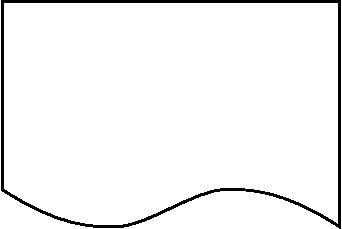
\includegraphics{styles/document.pdf}}}

\usepackage{epstopdf}

\tikzset{
  ciscorouter/.style={align=center,label={center:
      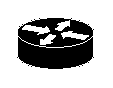
\includegraphics[]{styles/cisco/router.eps}
    },minimum width=0.9cm,minimum height=0.9cm}
}
\tikzset{
  ciscotap/.style={align=center,label={center:
      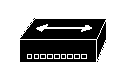
\includegraphics[]{styles/cisco/smallhub.eps}
    },minimum width=0.9cm,minimum height=0.9cm}
}

\usepackage{circuitikz}
\usepackage{multicol}
\newcommand*{\tabbox}[2][t]{\vspace{0pt}\parbox[#1][3.7\baselineskip]{1cm}{\strut#2\strut}}
\usepackage{float}
\usepackage{graphicx}
\usepackage{tabu}
\usepackage{lastpage}
\usepackage{lmodern}
\usepackage[toc,page]{appendix}
\usepackage[titles]{tocloft}
\usepackage{listings}
\usepackage{DejaVuSansMono}
\usepackage{tabularx}
\usepackage{fancyhdr}
\usepackage{cancel}
\setlength{\headheight}{15pt}
\pagestyle{fancyplain}
\usepackage{chngcntr}
\usepackage{footnote}
\makesavenoteenv{tabular}
\makesavenoteenv{table}
\counterwithout{footnote}{chapter}
\usepackage[hang,flushmargin,multiple]{footmisc}
\fancyhf{} % Ingen linje
% Skriv kapitelnavn som lowercase
\renewcommand{\chaptermark}[1]{\markboth{#1}{}}
\lhead[\fancyplain{}{\textit{\thechapter.\ \leftmark}}]{}
\rhead[]{\fancyplain{}{\textit{\leftmark\ \thechapter.}}}
\rfoot[]{\thepage}
\lfoot[\thepage]{}

\definecolor{lightgray}{gray}{0.90}
\newcommand{\colorbitbox}[3]{%
\rlap{\bitbox{#2}{\color{#1}\rule{\width}{\height}}}%
\bitbox{#2}{#3}}

\setcounter{tocdepth}{1}

%\renewcommand{\appendixname}{Bilag}
%\renewcommand{\appendixpagename}{Bilag}
%\renewcommand{\appendixtocname}{Bilag}

\usepackage{caption}
\captionsetup{font=footnotesize,labelfont=bf}
\captionsetup[figure]{labelfont=bf}
\usepackage{titlesec}
\titleformat{\chapter}{\normalfont\LARGE\bfseries}{\thechapter}{1em}{}
\titlespacing*{\chapter}{0pt}{-50pt}{20pt}
%\captionsetup[lstlisting]{labelfont=bf}
\usepackage{MnSymbol}
%\lstset{basicstyle=\scriptsize, tabsize=2, captionpos=b, frame=single}
\lstset{prebreak=\raisebox{0ex}[0ex][0ex]{\ensuremath{\rhookswarrow}}}
\lstset{breaklines=true, breakatwhitespace=true}
\renewcommand{\lstlistingname}{Code}

\lstset{
  language=c,
  basicstyle=\ttfamily\scriptsize,
  identifierstyle=\ttfamily,
  keywordstyle=\ttfamily,
  numbers=left,
  numbersep=5pt,
  xleftmargin=20pt,
  frame=tb,
  framexleftmargin=20pt,
  showstringspaces=false
}

\renewcommand*\thelstnumber{\arabic{lstnumber}:}

\DeclareCaptionFormat{mylst}{\hrule#1#2#3}
\captionsetup[lstlisting]{format=mylst,labelfont=bf,singlelinecheck=off,labelsep=space}


\usepackage{suffix}
\newcommand{\algoref}[1]{Algorithm~\ref{alg:#1}}
\newcommand{\appendixref}[1]{Appendix~-~\emph{\nameref{app:#1}}}
\newcommand{\appendixfigref}[2]{Appendix~\emph{\nameref{app:#1}~-~Figure~\ref{fig:#2}}}
\WithSuffix\newcommand\appendixref*[1]{Appendix~-~\emph{\nameref{app:#1}}}
%\newcommand{\@@appendixref}[1]{Appendix~\emph{\ref{app:#1}}}
\newcommand{\reqref}[1]{Req. \ref{req:#1_long}}
\newcommand{\reqrefnotext}[1]{Req. \ref{req:#1}}
\newcommand{\reqrefshort}[1]{\ref{req:#1_long}}
\newcommand{\reqrefshortnotext}[1]{\ref{req:#1}}
\captionsetup[subfigure]{labelformat=parens}
\newcommand{\subfigref}[1]{(\subref{fig:#1})}
\newcommand{\sectionref}[1]{Section~\emph{\ref{sec:#1}~\nameref{sec:#1}}}
\WithSuffix\newcommand\sectionref*[1]{Section~\emph{\ref{sec:#1}}}
\newcommand{\chapterref}[1]{Chapter~\emph{\ref{sec:#1}~\nameref{sec:#1}}}
\WithSuffix\newcommand\chapterref*[1]{Chapter~\emph{\ref{sec:#1}}}
\newcommand{\figref}[1]{Figure~\ref{fig:#1}}
\newcommand{\listingref}[1]{\lstlistingname~\ref{lst:#1}}
\newcommand{\tableref}[1]{Table~\ref{tab:#1}}
\newcommand{\theoremref}[1]{Theorem~\ref{th:#1}}
\newcommand{\equationref}[1]{Equation~\ref{eq:#1}}


\newcounter{req_counter}
\setcounter{req_counter}{1}

\makeatletter
\newcommand{\reqlabel}[2]{%
  \label{#1}
  \protected@write \@auxout {}{\string \newlabel {#1_long}{{\ref{#1} (#2)}{\thepage}{#2}{#1}{}}}%
  \hypertarget{#1}{#2}
}
\makeatother

\newcommand{\fullfigure}[3]{
  \begin{figure}[ht]
    \centering
    \includegraphics[width=.95\textwidth]{#1}
    \caption{#3}
    \label{fig:#2}
  \end{figure}
}

\newcommand{\fullfigurehere}[3]{
  \begin{figure}[H]
    \centering
    \includegraphics[width=.95\textwidth]{#1}
    \caption{#3}
    \label{fig:#2}
  \end{figure}
}

\newcommand{\fullfigureimport}[3]{
  \begin{figure}[ht]
    \centering
    \input{#1}
    \ifthenelse{\equal{#3}{}}{}{
      \caption{#3}
    }
    \ifthenelse{\equal{#2}{}}{}{
      \label{fig:#2}
    }
  \end{figure}
}

\newcommand{\largefigureimport}[3]{
  \begin{figure}[ht]
    \centering
    \scalebox{0.8}{\input{#1}}
    \ifthenelse{\equal{#3}{}}{}{
      \caption{#3}
    }
    \ifthenelse{\equal{#2}{}}{}{
      \label{fig:#2}
    }
  \end{figure}
}

\newcommand{\mediumfigureimport}[3]{
  \begin{figure}[ht]
    \centering
    \scalebox{0.66}{\input{#1}}
    \ifthenelse{\equal{#3}{}}{}{
      \caption{#3}
    }
    \ifthenelse{\equal{#2}{}}{}{
      \label{fig:#2}
    }
  \end{figure}
}

\newcommand{\smallfigureimport}[3]{
  \begin{figure}[ht]
    \centering
    \scalebox{0.50}{\input{#1}}
    \ifthenelse{\equal{#3}{}}{}{
      \caption{#3}
    }
    \ifthenelse{\equal{#2}{}}{}{
      \label{fig:#2}
    }
  \end{figure}
}

\newcommand{\tinyfigureimport}[3]{
  \begin{figure}[ht]
    \centering
    \scalebox{0.25}{\input{#1}}
    \ifthenelse{\equal{#3}{}}{}{
      \caption{#3}
    }
    \ifthenelse{\equal{#2}{}}{}{
      \label{fig:#2}
    }
  \end{figure}
}

\newcommand{\fullfigureimporthere}[3]{
  \begin{figure}[H]
    \centering
    \input{#1}
    \ifthenelse{\equal{#3}{}}{}{
      \caption{#3}
    }
    \ifthenelse{\equal{#2}{}}{}{
      \label{fig:#2}
    }
  \end{figure}
}

\newcommand{\fullfigureimporttop}[3]{
  \begin{figure}[t]
    \centering
    \input{#1}
    \ifthenelse{\equal{#3}{}}{}{
      \caption{#3}
    }
    \ifthenelse{\equal{#2}{}}{}{
      \label{fig:#2}
    }
  \end{figure}
}

\newcommand{\fullpagefigure}[3]{
  \begin{figure}[hbtp]
    \centering
    \includegraphics{#1}
    \caption{#3}
    \label{fig:#2}
  \end{figure}
}


\newcommand{\fullpagefigureimport}[3]{
  \begin{figure}[hbtp]
    \centering
    \input{#1}
    \caption{#3}
    \label{fig:#2}
  \end{figure}
}

\newcommand{\smallfigure}[3]{
  \begin{figure}[ht]
    \centering
    \includegraphics[width=.55\textwidth,height=.55\textwidth,keepaspectratio]{#1}
    \caption{#3}
    \label{fig:#2}
  \end{figure}
}

\newcommand{\smallerfigure}[3]{
  \begin{figure}[ht]
    \centering
    \includegraphics[width=.50\textwidth,height=.55\textwidth,keepaspectratio]{#1}
    \caption{#3}
    \label{fig:#2}
  \end{figure}
}

\newcommand{\tinyfigure}[3]{
  \begin{figure}[ht]
    \centering
    \includegraphics[width=.25\textwidth,height=.25\textwidth,keepaspectratio]{#1}
    \caption{#3}
    \label{fig:#2}
  \end{figure}
}


\newcommand{\mediumfigure}[3]{
  \begin{figure}[ht]
    \centering
    \includegraphics[width=.65\textwidth,height=.65\textwidth,keepaspectratio]{#1}
    \caption{#3}
    \label{fig:#2}
  \end{figure}
}

\newcommand{\largefigure}[3]{
  \begin{figure}[ht]
    \centering
    \includegraphics[width=.75\textwidth,height=.75\textwidth,keepaspectratio]{#1}
    \caption{#3}
    \label{fig:#2}
  \end{figure}
}

\newcommand{\largerfigure}[3]{
  \begin{figure}[ht]
    \centering
    \includegraphics[width=.85\textwidth,height=.85\textwidth,keepaspectratio]{#1}
    \caption{#3}
    \label{fig:#2}
  \end{figure}
}

\newcommand{\evenlargerfigure}[3]{
  \begin{figure}[ht]
    \centering
    \includegraphics[width=.99\textwidth,height=.95\textwidth,keepaspectratio]{#1}
    \caption{#3}
    \label{fig:#2}
  \end{figure}
}

\newcommand{\largestfigure}[3]{
  \begin{figure}[ht]
    \centering
    \includegraphics[width=1.05\textwidth,height=1.05\textwidth,keepaspectratio]{#1}
    \caption{#3}
    \label{fig:#2}
  \end{figure}
}


% \twofigures{width}{fig1name}{fig1label}{fig1caption}{fig2name}{fig2label}{fig2caption}{overall_label}{overall_caption}
\newcommand{\twofigures}[9]{
  \begin{figure}[H]
	\centering
	\begin{subfigure}[b]{#1\textwidth}
		\centering
		\includegraphics[width=\textwidth]{#2}
		\caption{#4}
        \label{fig:#3}
	\end{subfigure}
    \quad
	\begin{subfigure}[b]{#1\textwidth}
		\centering
		\includegraphics[width=\textwidth]{#5}
		\caption{#7}
        \label{fig:#6}
	\end{subfigure}
	\caption{#9}
    \label{fig:#8}
  \end{figure}
}

% \threefigures{width}{fig1name}{fig1caption}{fig2name}{fig2caption}{fig3name}{fig3caption}{fig4name}{fig4caption}{fig5name}{fig5caption}{overall_label}{overall_caption}
\newcommand{\threefigures}[9]{
  \begin{figure}[H]
	\centering
	\begin{subfigure}[b]{#1\textwidth}
		\centering
		\includegraphics[width=\textwidth]{#2}
		\caption{#3}
        \label{fig:#2}
	\end{subfigure}
    \quad
	\begin{subfigure}[b]{#1\textwidth}
		\centering
		\includegraphics[width=\textwidth]{#4}
		\caption{#5}
        \label{fig:#4}
	\end{subfigure}
    \quad
	\begin{subfigure}[b]{#1\textwidth}
		\centering
		\includegraphics[width=\textwidth]{#6}
		\caption{#7}
        \label{fig:#6}
	\end{subfigure}
	\caption{#9}
    \label{fig:#8}
  \end{figure}
}



% Bibliography
\bibliographystyle{IEEE}

\usepackage[footnote,draft,danish,silent,nomargin]{fixme}
\newcommand{\unit}[1]{~\text{#1}}
\newcommand{\rom}[1]{\uppercase\expandafter{\romannumeral #1}}

% colored hyperlinks
\newcommand{\chref}[2]{%
  \href{#1}{{\usebeamercolor[bg]{AAUsimple}#2}}%
}
\captionsetup{compatibility=false}
\title{Optimisation of Convolutional Neural Networks for Super-Resolution on Face Images}

%\subtitle{Super-Resolution}  % could also be a conference name

\date{June 28, 2016}

\author[]{
  Andreas Aakerberg, Malte Pedersen, Christoffer B. Rasmussen\\
  16gr843@es.aau.dk
}

% - Give the names in the same order as they appear in the paper.
% - Use the \inst{?} command only if the authors have different
%   affiliation. See the beamer manual for an example

\institute[]{% is placed on the bottom of the title page
  Vision, Graphics and Interactive Systems\\
  Aalborg University
  %there must be an empty line above this line - otherwise some unwanted space is added between the university and the country (I do not know why;( )
}

% specify a logo on the titlepage (you can specify additional logos an include them in 
% institute command below
\pgfdeclareimage[height=1.5cm]{titlepagelogo}{AAUgraphics/aau_logo_new} % placed on the title page
%\pgfdeclareimage[height=1.5cm]{titlepagelogo2}{AAUgraphics/aau_logo_new} % placed on the title page
\titlegraphic{% is placed on the bottom of the title page
  \pgfuseimage{titlepagelogo}
%  \hspace{1cm}\pgfuseimage{titlepagelogo2}
}

\begin{document}
% the titlepage
{\aauwavesbg%
\begin{frame}[plain,noframenumbering] % the plain option removes the header from the title page
  \titlepage
\end{frame}}

\begin{frame}{Agenda}{}
\tableofcontents
\end{frame}

%input{sections/intro.tex}
%\section{Problem Analysis}
% motivation for creating this theme
\begin{frame}{Main Challenges}{Object Variations}
\begin{columns}
    \column{0.2\textwidth}
        \begin{block}{Intra-class}
        \begin{itemize}
            \item Texture
            \item Colour
            \item Shape
            \item Size
        \end{itemize}
            

        \end{block}
    \column{0.4\textwidth}
        \begin{figure}
            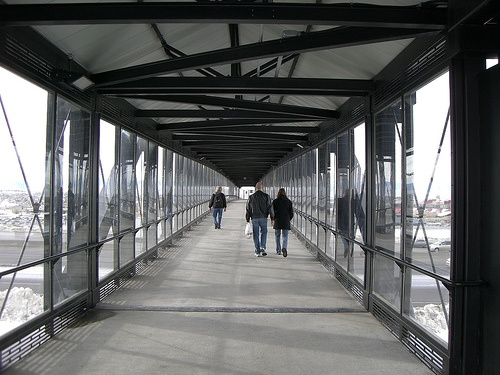
\includegraphics[width=0.7 \textwidth]{figs/000066.jpg}
        \end{figure}
        \begin{figure}
            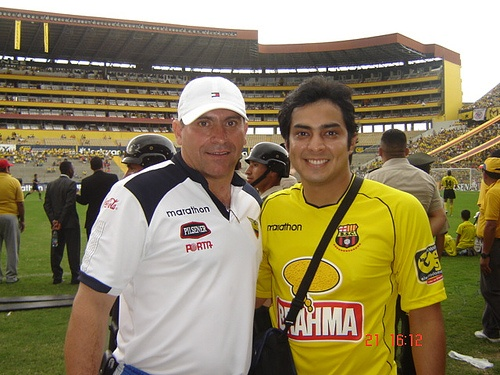
\includegraphics[width=0.7 \textwidth]{figs/000076.jpg}
        \end{figure}

    \column{0.4\textwidth}
        \begin{figure}
            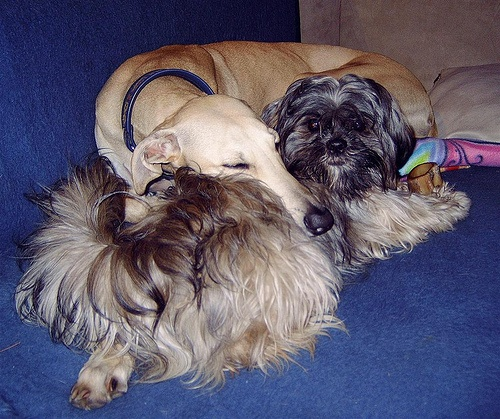
\includegraphics[width=0.7 \textwidth]{figs/000078.jpg}
        \end{figure}

    \end{columns}
\end{frame}

\begin{frame}{Main Challenges}{Object Variations}
\begin{columns}
    \column{0.2\textwidth}
        \begin{block}{Inter-class}
        \begin{itemize}
            \item Texture
            \item Colour
            \item Shape
            \item Size
        \end{itemize}
            

        \end{block}
    \column{0.4\textwidth}
        \begin{figure}
            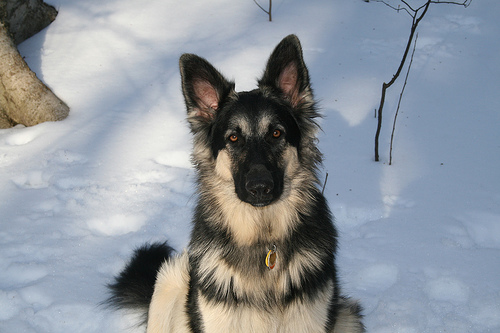
\includegraphics[width=1.0 \textwidth]{figs/germanshepherd.jpeg}
        \end{figure}
    \column{0.4\textwidth}
        \begin{figure}
            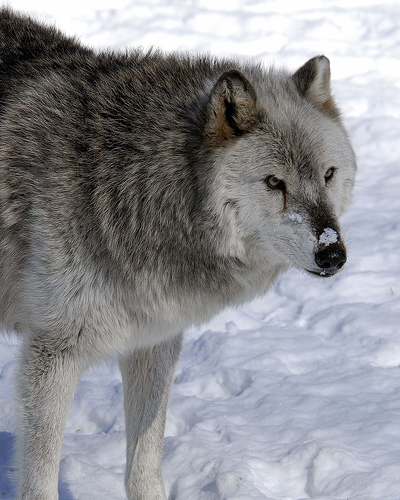
\includegraphics[width=0.7 \textwidth]{figs/wolf.jpeg}
        \end{figure}
    \end{columns}
\end{frame}

\begin{frame}{Main Challenges}{Image Variations}
\begin{columns}
    \column{0.3\textwidth}
        \begin{block}{Intra-class}
        \begin{itemize}
            \item Lighting
            \item Viewpoint
            \item Occlusion
            \item Clutter
            \item Quality
        \end{itemize}
            

        \end{block}
    \column{0.35\textwidth}
        \begin{figure}
            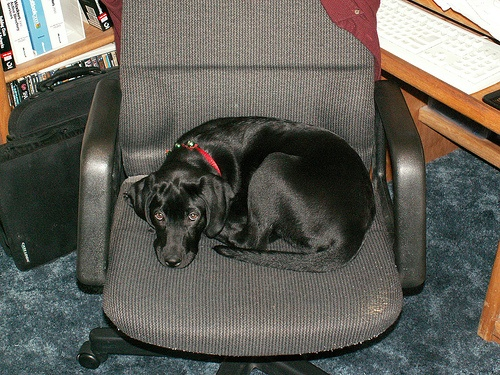
\includegraphics[width=0.7 \textwidth]{figs/000063.jpg}
        \end{figure}
        \begin{figure}
            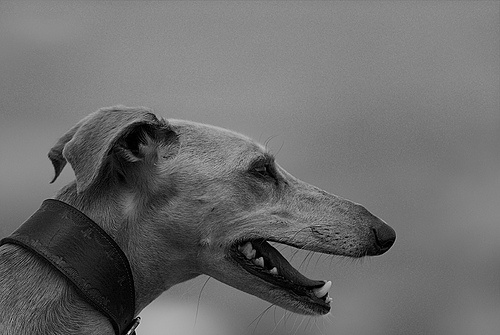
\includegraphics[width=0.7 \textwidth]{figs/000065.jpg}
        \end{figure}

    \column{0.35\textwidth}
        \begin{figure}
            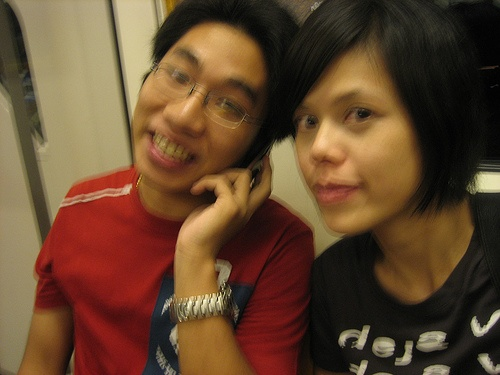
\includegraphics[width=0.7 \textwidth]{figs/000323.jpg}
        \end{figure}
        \begin{figure}
            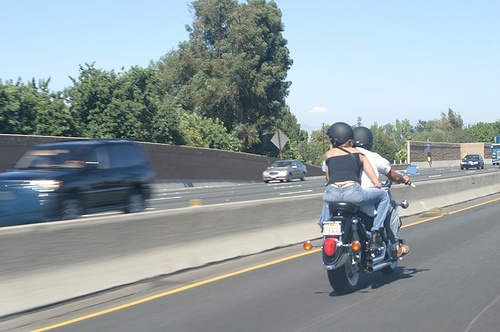
\includegraphics[width=0.7 \textwidth]{figs/000579.jpg}
        \end{figure}

    \end{columns}
\end{frame}


%\section{Ensemble Design}
% motivation for creating this theme
\begin{frame}{Designing the Ensemble}{R-FCN ResNet-101}
    \begin{block}{Overview}
    \begin{itemize}
        \item Ensemble of R-FCNs with ResNet-101
    \end{itemize}
    \begin{enumerate}
        \item Data sampling \& selection
        \begin{itemize}
            \item Object resolution
            \item Image quality
        \end{itemize}
        \item Training member classifiers
        \begin{itemize}
            \item Kept constant
        \end{itemize}
        \item Combining ensemble members
        \begin{itemize}
            \item Average
            \item Weighted Average
        \end{itemize}       
    \end{enumerate}
\end{block}
\end{frame}

\begin{frame}{Designing the Ensemble}{Pipeline}
    \begin{figure}
        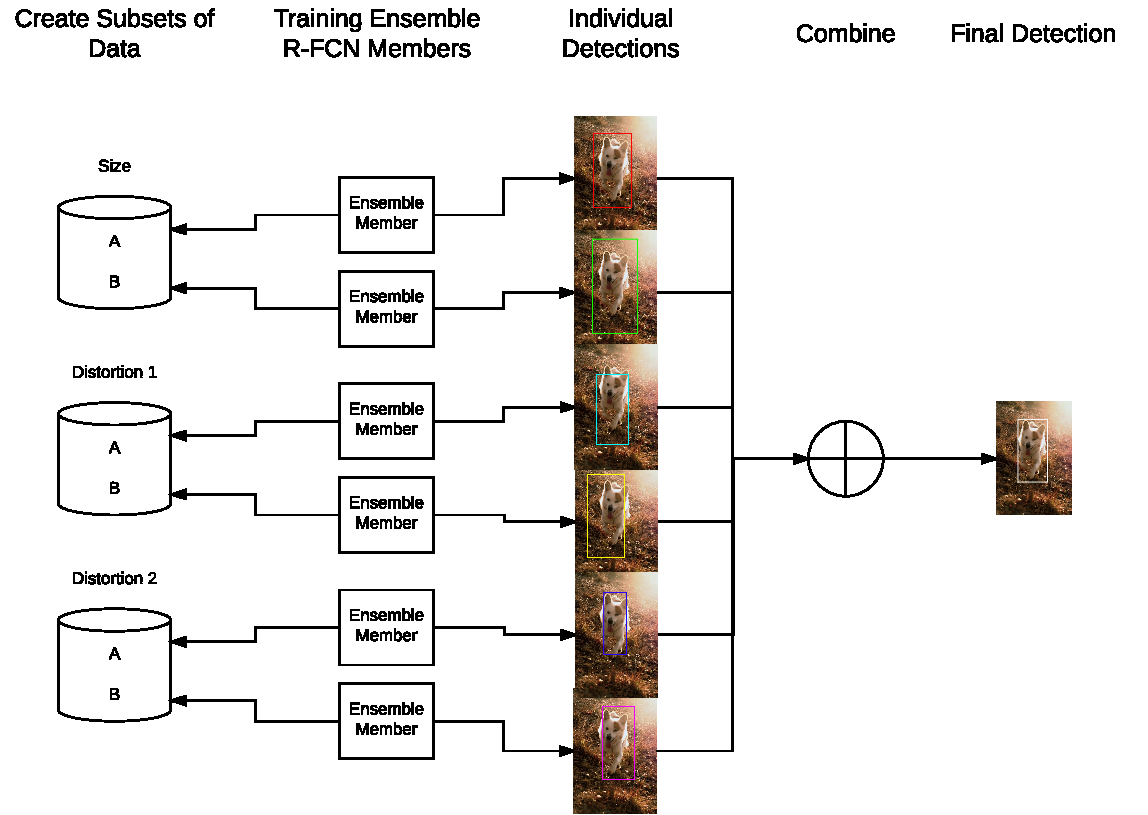
\includegraphics[width=0.8 \textwidth]{figs/ensembledesign.pdf}
    \end{figure}
\end{frame}

\begin{frame}{Training R-FCNs}{Ensemble Members}
\begin{columns}
    \column{0.5\textwidth}
        \begin{block}{Multi-step training}
        \begin{itemize}
            \item Train classifier with proposal inputs
            \item Ensure ensemble members infer from same input
            \item Simplify training process
        \end{itemize}
    \end{block}
    \column{0.5\textwidth}
        \begin{figure}
            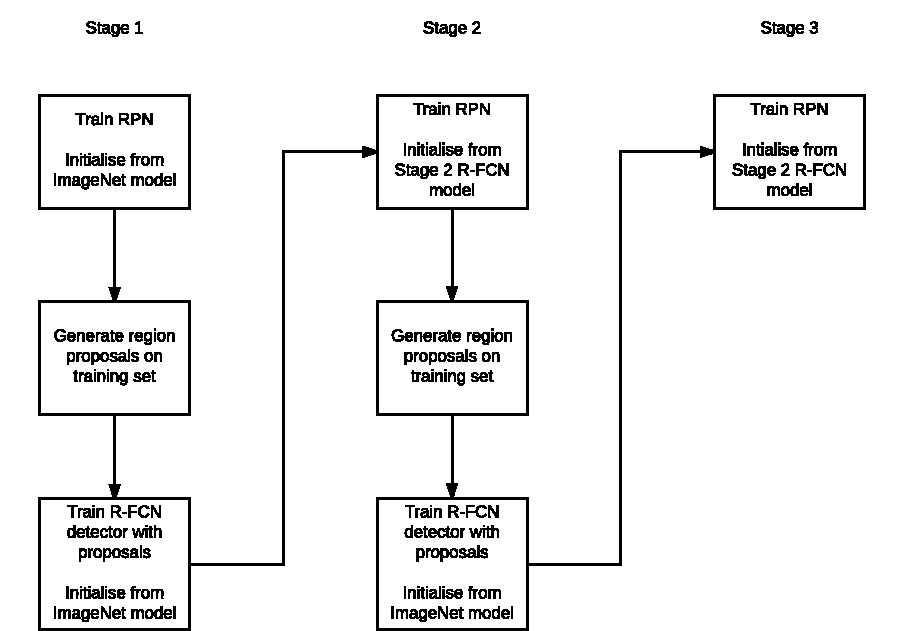
\includegraphics[width=1.0 \textwidth]{figs/4step-crop.pdf}
        \end{figure}
    \end{columns}
\end{frame}

\begin{comment}
	%%%%Overview%%%%
	- fundamental problem in CV
		- much work over previous decades
	- goal: find specific category in a given image
		- of interest by itself. Localise and classification
		- also a pre-requisite step to higher-level vision tasks
			- activity & event recognition, scene understanding, + find more
	- difficulties 
		- inter-class differences small
		- intra-class variations large
			- shape, pose, colour, texture, background, differences in illumination/viewpoint etc between images
	- GPU/deep learning advances have meant that performance is starting to become satisfactory for real-world use in scenarios requiring high precision and accuracy
		- autonomous vehicles, military, medicinal
	- much discussion of AI taking labor jobs
		- find articles and specific examples
			- elon musk, bill gates, etc (leaders of tech)
		- object detection needed
		- improvements still to be made before being completely realised
	- next section, overview of object detection definition, key task and challenges within. Also SOTA related work
\end{comment}


Object detection is a fundamental area of computer vision that has had a great amount of research over the past decades. The general goal of object detection is to find a specific object in an image. The specific object is typically from within a pre-defined list of categories that are of interest for a given use case. Object detection generally consists of two larger tasks; localisation and classification. It is assumed that the objects of interest are not already located in the image and as objects can vary in number of pixels depending on factors such as distance and scale, objects must be both localised in an image and classified accurately. Localisation is typically done by with a bounding-box indicating where a given object is in the image. However, other methods such as objects' centres and closed boundaries can also be used \cite{zhang}. Not only is object detection an important task in localising and classifying, it is also a necessary earlier step in larger computer vision pipelines. For example, object detection is needed within the tasks such as activity and event recognition, scene understanding, and robotic picking.

Object detection is a challenging problem due to both some large scale issues and minute differences. Firstly, there is the challenge of differentiating objects between classes. Depending on the problem at hand the sheer number of potential categories present can be into the thousands or tens of thousand. On top of this separate object categories can be both very different in appearance, for example an apple and an aeroplane, but separate categories can also be similar in appearance, such as dogs and wolves.

Current state-of-the-art within object detection is also within the realm of deep learning with \glspl{cnn}. This is exemplified with almost all leading entries in benchmark challenges such as \gls{pascalvoc} \cite{pascalvoc2012}, ImageNet \cite{imagenet}, and \gls{mscoco} \cite{mscoco} consisting of \gls{cnn}-based approaches. However, improvements are still needed before object detection can be used in real-world scenarios that require a high level of precision, accuracy, and performance. 

\section{Initial Problem Statement}

\begin{comment}
	- what are specific problems within object detection?
	- 
\end{comment}

An initial problem statement can be formed as follows: \\

\textit{How is object detection performed with \glspl{cnn}?} \\ \\
Based upon this, the following chapter will cover these challenges. On top of this, related work into current state-of-the-art object detection will be researched.

\section{Super Resolution}
% motivation for creating this theme
\begin{frame}{Super Resolution}{}
    \begin{block}{Increase spatial resolution to create a more detailed image.}

        \begin{figure}[H]
            \centering
            \begin{subfigure}[b]{0.25\textwidth}
                \includegraphics[width=\textwidth]{figs//butterfly_low.jpg}
                \caption*{\scriptsize LR image}
            \end{subfigure}
            \quad
            \begin{subfigure}[b]{0.25\textwidth}
                \includegraphics[width=\textwidth]{figs/butterfly_high.jpg}
                \caption*{\scriptsize HR image}
            \end{subfigure}
        \end{figure}

        \begin{itemize}
            \item Direct solution: Increase pixel density of the image sensor.
            \item Super-Resolution: Transform one or more LR images into a HR image.
        \end{itemize}


    \end{block}
\end{frame}




\begin{frame}{Super Resolution}{}
    \begin{block}{Pros (P) and cons (C) of increasing sensor resolution vs. performing Super Resolution}
        ~\\
        \begin{columns}
            \begin{column}{0.5\textwidth}
                \textbf{Increasing sensor resolution}
                \begin{itemize}
                    \item \textbf{P} - Actual increase of resolution/details.
                    \item \textbf{C} - Expensive and cumbersome.
                    \item \textbf{C} - Higher requirements to storage capacity.
                    \item \textbf{C} - Can introduce noise and blur.
                \end{itemize}
            \end{column}
            \begin{column}{0.5\textwidth}
                \textbf{Performing SR}
                \begin{itemize}
                    \item \textbf{P} - A generic cost effective solution.
                    \item \textbf{P} - Can be used only when needed to limit storage needs.
                    \item \textbf{C} - Enhancement is a "guess".
                    \item \textbf{C} - SoTA methods are still limited.
                \end{itemize}

            \end{column}
        \end{columns}




    \end{block}
\end{frame}




\begin{frame}{Super Resolution}{}


    \begin{block}{Super-Resolution methods:}

        \begin{itemize}
            \item Multiple image methods, based on sub-pixel shifts between LR-images.
            \item Single image methods, typically learning based.
        \end{itemize}

        \centering
        \begin{columns}
            \begin{column}{0.5\textwidth}
                \textbf{SoTA Super-Resolution:} Deep Learning, scientific computing accelerated using GPUs.
            \end{column}
            \begin{column}{0.5\textwidth}

                \includegraphics[width=0.5\textwidth]{figs/tesla.jpg}\footnotemark
            \end{column}
        \end{columns}
        \footnotetext{Image source: http://www.nvidia.com/object/tesla-workstations.html}
    \end{block}
\end{frame}


\section{Problem Statement}
% motivation for creating this theme
\begin{frame}{Problem Statement}{}


    \begin{block}{}

        Based on the SoTA super-resolution convolutional neural network, SRCNN, by Dong et al., we aim to investigate the following:\\
        ~\\


        \textit{How can a state-of-the-art CNN based SR algorithm be enhanced to create images of higher quality?}
        \begin{itemize}
            \item How does a SRCNN optimised to specific image types, such as faces, perform?
            \item How does a SRCNN combined with a classic SR method perform?
        \end{itemize}


    \end{block}
\end{frame}




\section{Dataset}
% motivation for creating this theme
\begin{frame}{Dataset}{}


    \begin{block}{}

        Training datasets of face images are needed as the SRCNN is a learning based super-resolution method.

        \begin{table}[]
            \resizebox{\textwidth}{!}{

                \begin{tabular}{|l|l|l|l|}
                    \hline
                    & \textbf{AR500}     & \textbf{AToF}       & \textbf{LFD}   \\ \hline
                    \textbf{Characteristics} & Similar conditions & Very large variation & Large variation \\ \hline
                    \textbf{Images}          & 500                & 153                 & 13300          \\ \hline
                \end{tabular}
            }
        \end{table}

        Several test datasets are also used (AR5, TDRF and SET5).
    \end{block}
\end{frame}


\begin{frame}{Dataset}{}
    \begin{block}{}
        \vspace{-1cm}
        \begin{columns}
            \begin{column}{0.1\textwidth}
                AR500\\
                ~\\
                ~\\
                ~\\
                AToF\\
                ~\\
                ~\\
                ~\\
                LFD
            \end{column}
            \hspace{-1cm}
            \begin{column}{1\textwidth}
                \begin{figure}[H]
                    \begin{subfigure}[b]{0.1\textwidth}
                        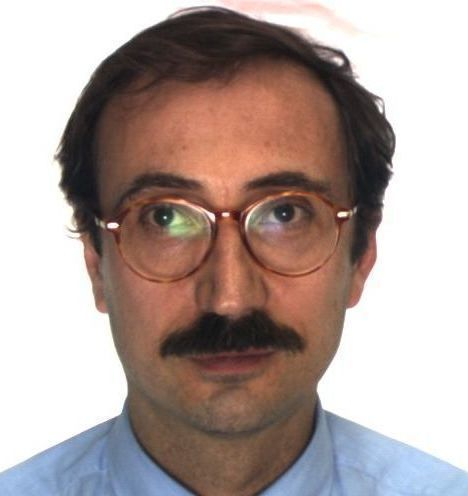
\includegraphics[width=\textwidth]{figs/ar1.jpg}
                    \end{subfigure}
                    \quad
                    \begin{subfigure}[b]{0.1\textwidth}
                        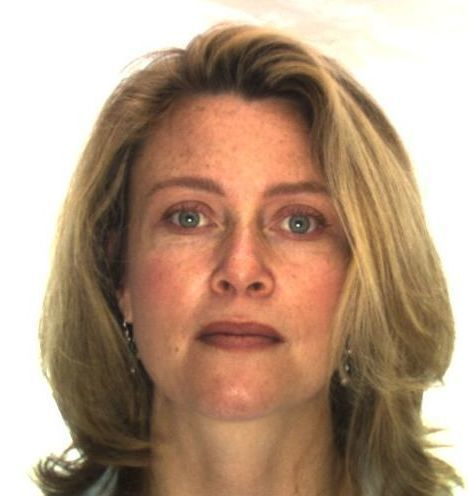
\includegraphics[width=\textwidth]{figs/ar2.jpg}
                    \end{subfigure}
                    \quad
                    \begin{subfigure}[b]{0.1\textwidth}
                        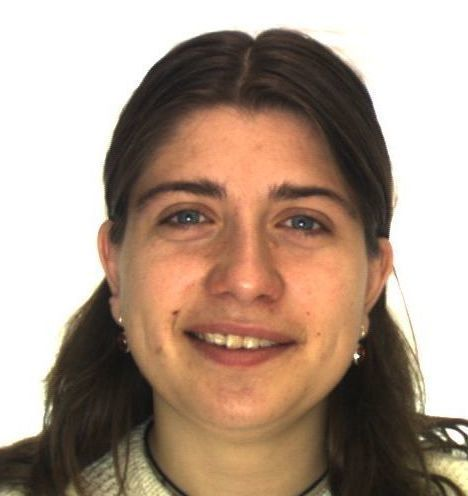
\includegraphics[width=\textwidth]{figs/ar3.jpg}
                    \end{subfigure}
                    \quad
                    \begin{subfigure}[b]{0.1\textwidth}
                        \includegraphics[width=\textwidth]{figs/ar4.jpg}
                    \end{subfigure}
                    \quad
                    \begin{subfigure}[b]{0.1\textwidth}
                        \includegraphics[width=\textwidth]{figs/ar5.jpg}
                    \end{subfigure}
                \end{figure}


                \begin{figure}[H]
                    \begin{subfigure}[b]{0.1\textwidth}
                        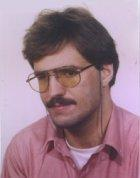
\includegraphics[width=\textwidth]{figs/atof1.jpg}
                    \end{subfigure}
                    \quad
                    \begin{subfigure}[b]{0.1\textwidth}
                        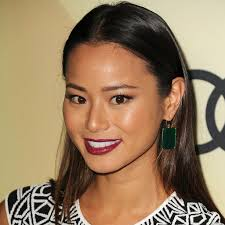
\includegraphics[width=\textwidth]{figs/atof2.jpg}
                    \end{subfigure}
                    \quad
                    \begin{subfigure}[b]{0.1\textwidth}
                        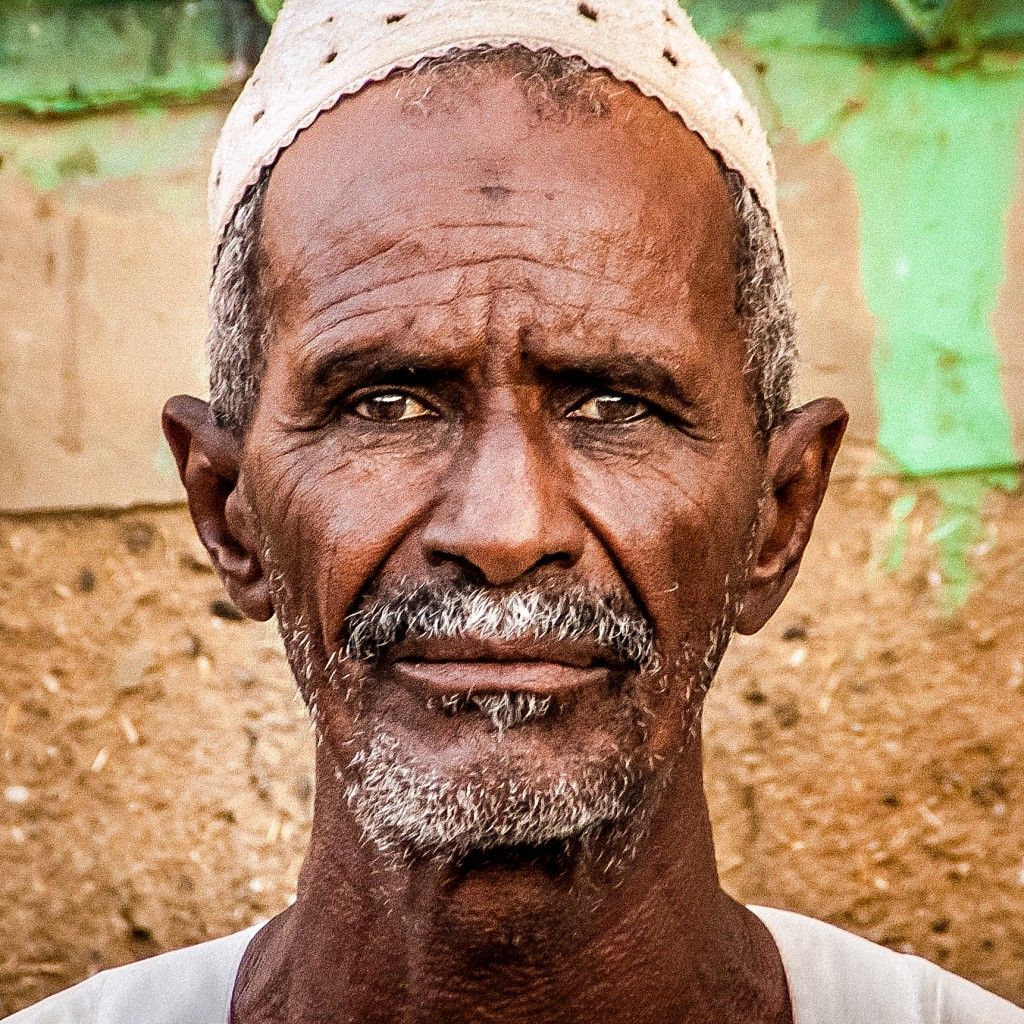
\includegraphics[width=\textwidth]{figs/atof3.jpg}
                    \end{subfigure}
                    \quad
                    \begin{subfigure}[b]{0.1\textwidth}
                        \includegraphics[width=\textwidth]{figs/atof4.jpg}
                    \end{subfigure}
                    \quad
                    \begin{subfigure}[b]{0.1\textwidth}
                        \includegraphics[width=\textwidth]{figs/atof5.jpg}
                    \end{subfigure}
                \end{figure}

                \begin{figure}[H]
                    \begin{subfigure}[b]{0.1\textwidth}
                        \includegraphics[width=\textwidth]{figs/lfd1.jpg}
                    \end{subfigure}
                    \quad
                    \begin{subfigure}[b]{0.1\textwidth}
                        \includegraphics[width=\textwidth]{figs/lfd2.jpg}
                    \end{subfigure}
                    \quad
                    \begin{subfigure}[b]{0.1\textwidth}
                        \includegraphics[width=\textwidth]{figs/lfd3.jpg}
                    \end{subfigure}
                    \quad
                    \begin{subfigure}[b]{0.1\textwidth}
                        \includegraphics[width=\textwidth]{figs/lfd4.jpg}
                    \end{subfigure}
                    \quad
                    \begin{subfigure}[b]{0.1\textwidth}
                        \includegraphics[width=\textwidth]{figs/lfd5.jpg}
                    \end{subfigure}
                \end{figure}


            \end{column}

        \end{columns}




    \end{block}
\end{frame}



As covered in \sectionref{related}, the current leading methods in object detection are within the domain of deep learning. This chapter will cover the core concepts of deep learning which will include general architecture of \glspl{cnn}, typical layers and optimisation strategies. Also covered will be aspects of deep learning that are more specific to object detection with \glspl{cnn}.

\section{Convolutional Neural Networks}
\glspl{cnn} are an extension of artificial neural networks which have existed for decades. Neural networks consist of neurons that receive inputs and have learned parameters such that the input can be altered in some manner. In the neuron, the dot product is computed between the input and parameters. For \glspl{cnn}, the key difference is the first input to the network is an image and the parameters in the neurons are filters which are trained to activate towards certain inputs. One of the first successful \gls{cnn} methods was LeNet for hand-written digit classification in 1989 \cite{lenet}. However, after this point, deep learning research became stagnant mostly due to the large amount of processing needed in training. The return of deep learning is often attributed to AlexNet in 2012 \cite{alexnet}, which gave significant improvements in image classification on ImageNet.
\\\\
The general architecture of a \gls{cnn} is shown in \figref{generalcnn}. The network takes an image as input, this can be a single channel as depicted in the figure or multiple such as an colour image. Convolutional operations with learned filters are applied to an area of the input image dependent on the filter size to produce an output at a given layer shown by the red dot. The size of the filters at a given layer constitutes the receptive field of that layer. For example, a 9$\times$9 filter has a larger receptive field than a 3$\times$3 filter to produce a given response. Each filter is individually trained and shown as the arrows leading to the dots. In the second convolutional layer is where the network starts to be considered deep. Again, convolutional operations are performed to produce an output. Depending on the architecture of the network many convolutional layers can be present, generally deeper networks are able to find richer abstract features for the given task. Finally the network may have a fully-connected layer that produces confidence scores. These scores can be used to determine how well an input image represents a given class for a classification problem.

\begin{figure}[H]
  \centering
    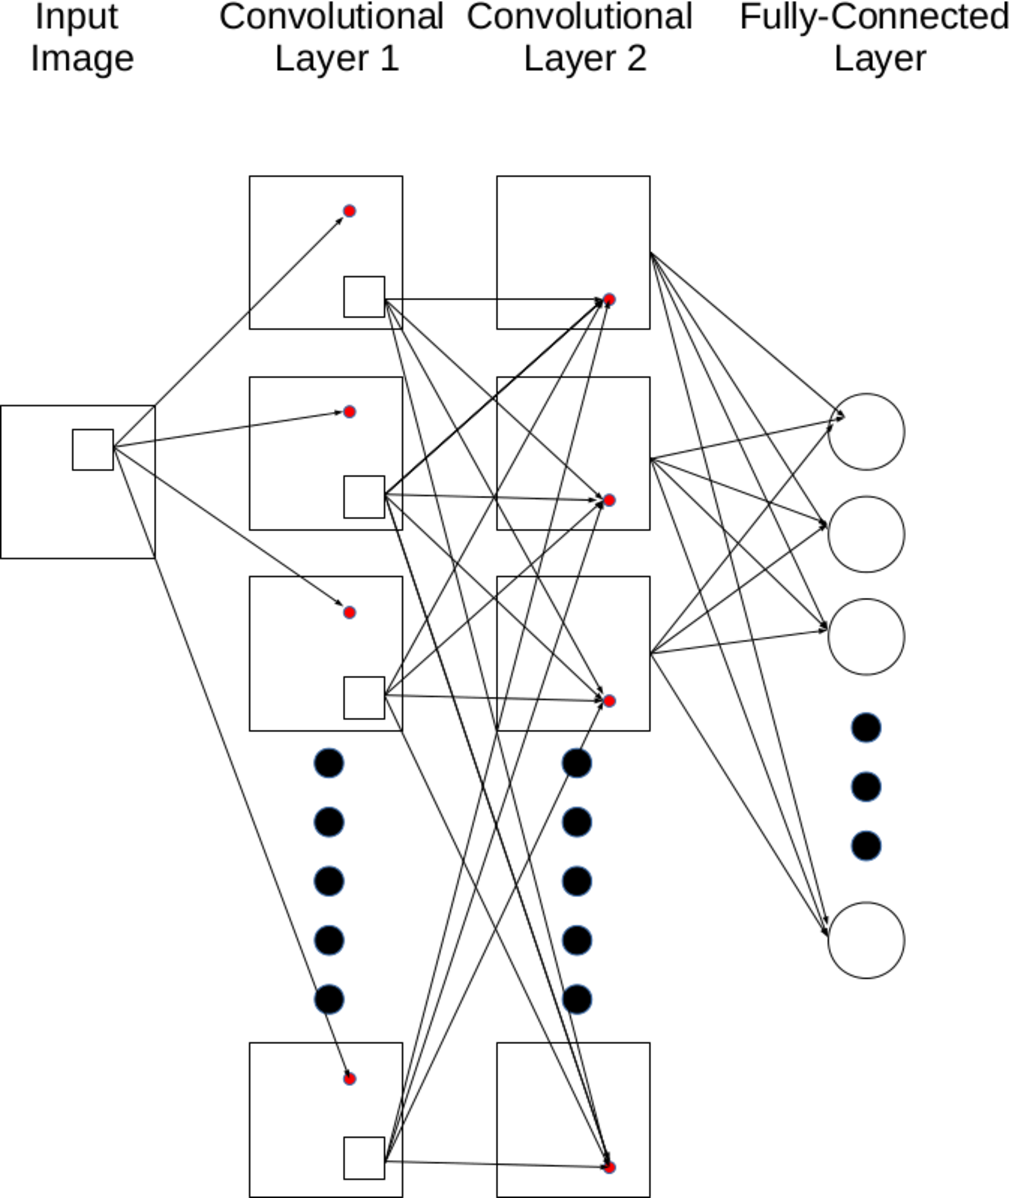
\includegraphics[width=0.6\textwidth]{Figs/Techanal/cnnarch.pdf}
      \caption{An example of a general \gls{cnn} with convolutional and fully-connected layers.}
    \label{fig:generalcnn}
\end{figure}

The activation function within a convolutional layer is another key aspect to neural networks. The activation layer is used to add non-linearity to the network and measures how well a given convolutional operation and associated bias fires for a patch in either the input image or a previous layer. Typically activation functions output between 0 and 1 to represent this measurement. In earlier adaptations of \glspl{cnn} the a sigmoid activation function was popular to map the output of a convolutional layer between 0 and 1. However, most current \glspl{cnn} take advantage of the \glspl{relu} activation function. \gls{relu} is a simple thresholding function that maps negative outputs to 0 and positive outputs are kept unchanged.
\\\\
In order to learn the parameters in a \gls{cnn} an optimisation strategy is required. The training process is to minimise a loss function in respect the inputs. Typically the learning is done through gradient descent with backpropgation. The intuition here is to update parameters after each forward iteration such that the loss calculated between input samples and their labels is decreased. Generally for each forward pass the loss is calculated as the average loss over a mini-batch of samples. This is both more efficient and produces a less stochastic learning process. Once the loss is found the gradient indicates which direction to update parameters and this information is backpropagated right through to the initial parameters.
\\\\
A key aspect of training \glspl{cnn} is how the parameters in a network are initialised. Poor initialisation of parameters can make the training process slow or impossible if the initial operations fire the activation functions too violently. Common approaches to initialisation include sampling the weights from a Gaussian distribution and setting all biases to zero. Other alternative dynamic approaches do exist, such as Xavier initialisation \cite{xavier}. In this case the architecture of the network is measured, such as number of filters in a layer, and weights are sampled according to this information. Another initialisation method is fine-tuning parameters from a pre-trained network. A pre-trained network is typically trained on a large set of data and has learnt parameters to that given task, then by updating the parameters they can be changed towards a new task. This can provide a number of benefits. Firstly, the amount of training time can be drastically reduced as strong general parameters have already been learned. Also, if the amount of training data is sparse, fine-tuning can aid such that the risk of overfitting is reduced.

\documentclass{standalone}
\usepackage{tikz, xifthen, calc}
\usetikzlibrary{shapes.geometric, 3d, calc}
\def\inline{\lstinline[keywordstyle={}]}
\tikzstyle{img}=[]

\begin{document}
\begin{tikzpicture}[]

    \node (lr) [inner sep = 0, outer sep = 0, anchor = west, label=above:LR] at (-5., 5.5) {\includegraphics[width=20pt]{figs/lr_butterfly_GT.jpeg}};

    \node (hr) [inner sep = 0, outer sep = 0, anchor = west, label=above:LR input] at (-3.5, 5.5) {\includegraphics[width=60pt]{figs/bicubic_butterfly_GT.jpeg}};

\draw[->](lr) -- node[align=center,yshift=-1.7cm] {Bicubic\\Interpolation} (hr);

\draw[dotted] (-6,3) -- (-0.5,3) -- (-0.5,8) -- (-6,8) -- (-6, 3);
\node[] at (-4.6,8.5) {\textbf{Pre-processing}};

%\node (conv) at (1.7,5.5) [draw, label=above:Input Input, minimum width=2cm,minimum height=2cm] {};

\node (conv1) at (1.5,5.5) [draw,minimum width=2cm,minimum height=2cm] {};
\node (rect1) at (1.6,5.6) [draw,fill=white,minimum width=2cm,minimum height=2cm] {};
\node (convEnd1) at (1.7,5.7) [draw,fill=white,minimum width=2cm,minimum height=2cm] {};
\node[anchor=south,align=left]  at ([yshift=0.2cm]conv1.north) {Patch\\extraction}; 

\draw[->](hr) -- node[align=center,xshift=1.1cm, yshift=-2cm]{} (conv1);

\node (conv2) at (4.2,5.5) [draw,minimum width=2cm,minimum height=2cm] {};
\node (rect2) at (4.3,5.6) [draw,fill=white,minimum width=2cm,minimum height=2cm] {};
\node (convEnd2) at (4.4,5.7) [draw,fill=white,minimum width=2cm,minimum height=2cm] {};
\node[anchor=south,align=left] at ([yshift=0.18cm]conv2.north) {Non-linear\\mapping}; 

\draw[->](convEnd1) -- node[align=center, yshift=-2cm] {} (convEnd2);

\node (conv3) at (6.9,5.7) [draw,minimum width=2cm,minimum height=2cm] {};
\draw[->](convEnd2) -- node[align=center, yshift=-2cm] {} (conv3);
\node[anchor=south,align=left] at ([yshift=0.05cm,xshift=0.2cm]conv3.north) {Reconstruction};

\draw[dotted] (0.2,3) -- (8.8,3) -- (8.8,8) -- (0.2,8) -- (0.2,3);
\node[] at (0.8,8.5) {\textbf{SRCNN}};

\node (out) [inner sep = 0, outer sep = 0, anchor = west, label=above:HR output] at (9.2, 5.7) {\includegraphics[width=60pt]{figs/srcnn_butterfly_GT.jpeg}};

\draw[->](conv3) -- node[align=center, yshift=-2cm] {} (out);


\end{tikzpicture}
\end{document}

\section{Results}
% motivation for creating this theme
\begin{frame}{Results}{}
\begin{columns}
    \column{0.3\textwidth}
    \begin{block}{Ensemble strategies}
    \begin{itemize}
        \item No improvement vs baseline
    \end{itemize}  
\end{block}  
    \column{0.7\textwidth}
    \begin{table}[]
    \centering
    \begin{tabular}{|l|l|l|}
    \hline
    \textbf{Method} & \textbf{AP$_{report}$} & \textbf{AP$_{new}$} \\ \hline
    Average          & 79.21     & 79.45  \\ \hline
    Weighted Average & 79.13     & 79.47  \\ \hline
    Baseline         & \textbf{79.59}     & -  \\ \hline
    \end{tabular}
    \end{table} 

\end{columns}
\end{frame}

\begin{frame}{Results}{}
\begin{columns}
    \column{0.3\textwidth}
    \begin{block}{Ensemble strategies}
    \begin{itemize}
        \item Some strategies may not be suitable for factors
        \begin{itemize}
            \item IQA: weighted average
            \item Object resolution: average
        \end{itemize}    
    \end{itemize}  
    

\end{block} 
\column{0.7\textwidth} 
    \begin{table}[h]
    \centering
    \caption{Average}
    \begin{tabular}{|l|l|}
    \hline
    \textbf{Ensemble Members}        & \textbf{AP} \\ \hline
    Image Quality & 78.15 \\ \hline
    Resolution    & 78.13 \\ \hline
    \end{tabular}
    \end{table}

    \begin{table}[]
    \centering
    \caption{Weighted average}
    \begin{tabular}{|l|l|l|}
    \hline
     \textbf{Ensemble Members} &  \textbf{AP$_{report}$} & \textbf{AP$_{new}$} \\ \hline
    Image Quality                                              & 78.44     & 79.04  \\ \hline
    Weighted Average                                           & 75.00     & 77.84  \\ \hline
    \end{tabular}
    \end{table}

\end{columns}
\end{frame}


\begin{frame}{Results}{}
    \begin{block}{Ensemble strategies}
    \begin{itemize}
        \item Combining with both strategies  
    \end{itemize}  
\end{block} 

    \begin{table}[]
    \centering
    \begin{tabular}{|l|l|l|}
    \hline
    \textbf{Ensemble Members} & \textbf{AP$_{report}$} & \textbf{AP$_{new}$} \\ \hline
    Image Quality$_{WAvg}$ / Resolution$_{Avg}$ avg                                          & 79.90     & 79.83  \\ \hline
    Image Quality$_{Avg}$ / Resolution$_{WAvg}$                                         & 78.71     & 79.17  \\ \hline
    Baseline                                                   & 79.59     & -      \\ \hline
    \end{tabular}
    \end{table}
\end{frame}

\begin{frame}{Results}{}
    \begin{block}{Ensemble strategies}
    \begin{itemize}
        \item Adding the baseline model
        \item All baseline detection weighted 1.0
        \item 0.56 AP improvement
    \end{itemize}  
\end{block} 
    \begin{table}[h]
    \centering
    \begin{tabular}{|l|l|l|}
    \hline
    \textbf{Ensemble Members}                  & \textbf{AP$_{report}$} & \textbf{AP$_{new}$} \\ \hline
    Image Quality$_{WAvg}$ / Resolution$_{Avg}$  & 79.90 & 79.83 \\ \hline
    Image Quality$_{WAvg}$ / Resolution$_{Avg}$ $_{base}$ & \textbf{80.15} & 80.09 \\ \hline
    Image Quality$_{Avg}$ / Resolution$_{WAvg}$ & 78.71 & 79.17 \\ \hline
    Image Quality$_{Avg}$ / Resolution$_{WAvg}$ $_{base}$ & 79.10 & 79.54\\ \hline
    Baseline                          & 79.59 & -\\ \hline
    \end{tabular}
    \end{table}
\end{frame}

\begin{frame}{Results}{}
    \begin{columns}
    \column{0.3\textwidth}
    \only<1>{
        \begin{block}{Demonstration of system}
        \end{block}
    }
    \only<2>{
        \begin{block}{Region proposal}
        \end{block}
    }
    \only<3>{
        \begin{block}{Gaussian blur detections}
        \begin{itemize}
            \item 4.807 deep IQA Gaussian blur
            \item Lower weight: 1.14
            \item Upper weight: 0.86
        \end{itemize}
        \end{block}
    }
    \only<4>{
        \begin{block}{Combined Gaussian blur}
        
        \end{block}
    }
    \only<5>{
        \begin{block}{Baseline added}
        
        \end{block}
    }
    \only<6>{
        \begin{block}{Fast fading}
        
        \end{block}
    }
    \only<7>{
        \begin{block}{JP2K}
        
        \end{block}
    }
    \only<8>{
        \begin{block}{JPEG}
        
        \end{block}
    }
    \only<9>{
        \begin{block}{Resolution}
        
        \end{block}
    }
    \only<10>{
        \begin{block}{Final combined detection}
        
        \end{block}
    }
    \only<11>{
        \begin{block}{Final combined detection}
        
        \end{block}
    }
    \only<12>{
        \begin{block}{Intersection-over-union}
        \begin{itemize}
            \item {\color{green}Ground truth}
            \item {\color{red}Baseline: 0.80}
            \item {\color{blue}Ensemble: 0.85}
        \end{itemize}
        \end{block}
    }
    
     
\column{0.7\textwidth} 
    \only<1>{
        \begin{figure}
            \includegraphics[width=0.9\textwidth]{figs/demo/000069_gt.jpg}
        \end{figure}
    }
    \only<2>{
        \begin{figure}
            \includegraphics[width=0.9\textwidth]{figs/demo/000069_proposal.jpg}
        \end{figure}
    }
    \only<3>{
        \begin{figure}
            \includegraphics[width=0.9\textwidth]{figs/demo/000069_blurboth.jpg}
        \end{figure}
    }
    \only<4>{
        \begin{figure}
            \includegraphics[width=0.9\textwidth]{figs/demo/000069_blurboth_comb.jpg}
        \end{figure}
    }
    \only<5>{
        \begin{figure}
            \includegraphics[width=0.9\textwidth]{figs/demo/000069_dets3.jpg}
        \end{figure}
    }
    \only<6>{
        \begin{figure}
            \includegraphics[width=0.9\textwidth]{figs/demo/000069_dets5.jpg}
        \end{figure}
    }
    \only<7>{
        \begin{figure}
            \includegraphics[width=0.9\textwidth]{figs/demo/000069_dets7.jpg}
        \end{figure}
    }
    \only<8>{
        \begin{figure}
            \includegraphics[width=0.9\textwidth]{figs/demo/000069_dets9.jpg}
        \end{figure}
    }
    \only<9>{
        \begin{figure}
            \includegraphics[width=0.9\textwidth]{figs/demo/000069_dets10.jpg}
        \end{figure}
    }
    \only<10>{
        \begin{figure}
            \includegraphics[width=0.9\textwidth]{figs/demo/000069_detfinal.jpg}
        \end{figure}
    }
    \only<11>{
        \begin{figure}
            \includegraphics[width=0.9\textwidth]{figs/demo/000069_detfinal2.jpg}
        \end{figure}
    }
    \only<12>{
        \begin{figure}
            \includegraphics[width=0.9\textwidth]{figs/demo/000069_detfinal2.jpg}
        \end{figure}
    }

\end{columns}

\end{frame}
\begin{comment}

\subsection{License}
% the license
\begin{frame}{Introduction}{License}
  \begin{itemize}
    \item<1-> The AAU logo is covered by copyright rules. I have used the logo from \chref{http://aau.designguiden.dk}{http://aau.designguiden.dk}. As long as you use the theme for making presentations in connection with your work at AAU, you are allowed to use the AAU logo.
    \item<2-> The rest of the theme is provided under the GNU General Public License v. 3 (GPLv3). This basically means that you can redistribute it and/or modify it under the same license. For more information on the GPL license see \chref{http://www.gnu.org/licenses/}{http://www.gnu.org/licenses/}
  \end{itemize}
\end{frame}
%%%%%%%%%%%%%%%%

\section{Installation}
% general installation instructions
\begin{frame}{Installation}
  The theme consists of four files
  \begin{enumerate}
    \item {\tt beamerthemeAAUsimple.sty}
    \item {\tt beamerinnerthemeAAUsimple.sty}
    \item {\tt beamerouterthemeAAUsimple.sty}
    \item {\tt beamercolorthemeAAUsimple.sty}
  \end{enumerate}
  The theme can either be installed for local or global use.
  \pause
  \begin{block}{Local Installation}
    The simplest way of installing the theme is by placing the four theme files in the same folder as your presentation. When you download the theme, the four theme files are located in the {\tt local} folder.
  \end{block}
\end{frame}

% general installation instructions
\begin{frame}{Installation}
  \begin{block}{Global Installation}
  \begin{itemize}
     \item If you wish to make the theme globally available, you must put the files in your local latex directory tree. The location of the root of the local directory tree depends on the operating system and the latex distribution. On the following slides, you can read the instructions for some common setups.
    \item When you download the theme, the four theme files are embedded in a directory structure (in the {\tt global} folder) ready to be copied directly to the root of your local directory tree.
    \item On the following slides, we refer to this directory structure as {\tt <dirstruct>}. \alert{Note} that some parts of the directory may already exist if you have installed other packages in your local latex directory tree. If this is the case, you simply merge {\tt <dirstruct>} with your existing setup.
  \end{itemize}
  \end{block}
\end{frame}

\subsection{GNU/Linux}
% installation on GNU/Linux
\begin{frame}{Installation}{GNU/Linux}
  \begin{block}{Ubuntu with TeX Live}
    \begin{enumerate}
      \item Place the {\tt <dirstruct>} in the root of your local latex directory tree. By default it is\\
        {\tt \textasciitilde /texmf}\\
        If the root does not exist, create it. The symbol {\tt \textasciitilde} refers to your home folder, i.e., {\tt /home/<username>}
      \item In a terminal run\\
        {\tt \$ texhash \textasciitilde /texmf}
    \end{enumerate}
  \end{block}
\end{frame}
%%%%%%%%%%%%%%%%

\subsection{Microsoft Windows}
% installation on Microsoft Windows
\begin{frame}{Installation}{Microsoft Windows}
  \begin{block}{Windows with MiKTeX}
    Apparently, MiKTeX does not include a local latex directory tree by default. Therefore, you first have to create it.
    \begin{enumerate}
      \item To do this, create a folder {\tt <somewhere>} named, e.g., {\tt texmf}
      \item Add this folder in the Roots tab of the MiKTeX Settings dialog
      \item Place the {\tt <dirstruct>} in your newly created local latex directory tree\\
    {\tt <somewhere>\textbackslash texmf}\\
      \item Open the MiKTeX Settings dialog and click Refresh FNDB.
    \end{enumerate}
  \end{block}
\end{frame}
%%%%%%%%%%%%%%%%

% installation on Microsoft Windows Cont'd
\begin{frame}{Installation}{Microsoft Windows}
  \begin{block}{Windows with TeX Live}
    In the advanced TeX Live Installer, you can manually change the default position of the root of the local latex directory tree. However, we assume the default position below.
    \begin{enumerate}
      \item Place the {\tt <dirstruct>} in your local latex directory tree\\
        {\tt \%USERPROFILE\%\textbackslash texmf}\\
        If it does not exist, create it. In XP {\tt \%USERPROFILE\%} is\\
      {\tt c:\textbackslash Document and Settings\textbackslash<username>}\\
      by default, and in Vista and above it is by default\\
      {\tt c:\textbackslash Users\textbackslash<username>}
      \item Open the TeX Live Manager dialog and select 'Update filename database' under 'Actions'.
    \end{enumerate}
  \end{block}
\end{frame}
%%%%%%%%%%%%%%%%

\subsection{Mac OS X}
% installation on Mac OS X
\begin{frame}{Installation}{Mac OS X}
  \begin{block}{Mac OS X with MacTeX}
     Place the {\tt <dirstruct>} in the root of your local latex directory tree. By default it is\\
        {\tt \textasciitilde /Library/texmf}\\
        If the root does not exist, create it. The symbol {\tt \textasciitilde} refers to your home folder, i.e., {\tt /home/<username>}
  \end{block}
\end{frame}
%%%%%%%%%%%%%%%%

\subsection{Required Packages}
% list of required packages
\begin{frame}{Installation}{Required Packages}
  Of course, you have to have the Beamer class installed. In addition, the theme loads two packages
  \begin{itemize}
    \item TikZ\footnote{By the way, TikZ is an awesome package for creating beautiful graphics. If you do not believe me, then have a look at these \chref{http://www.texample.net/tikz/examples/}{online examples} or the \chref{http://tug.ctan.org/tex-archive/graphics/pgf/base/doc/generic/pgf/pgfmanual.pdf}{pgf user manual}. If you want to create beautiful plots, you should use the pgfplots package which is based on TikZ.}
    \item calc
  \end{itemize}
  These packages are very common and should therefore be included in your latex distribution.
\end{frame}
%%%%%%%%%%%%%%%%

\section{User Interface}
\subsection{Loading the Theme and Theme Options}
% list of the themes and options
\begin{frame}{User Interface}{Loading the Theme and Theme Options}
  \begin{block}{The Presentation Theme}
    It is very simple to load the presentation theme. Just type\\
    {\tt \textbackslash usetheme[<options>]\{AAUsimple\}}\\
    which is exactly the same way other beamer presentation themes are loaded. The presentation theme loads the inner, outer and color AAU Simple theme files and passes the {\tt <options>} on to these files.
  \end{block}
  \begin{block}{The Inner Theme}
    You can load the inner theme directly by\\
    {\tt \textbackslash useinnertheme\{AAUsimple\}}\\
    and it has no options.
  \end{block}
\end{frame}
%%%%%%%%%%%%%%%%

% list of the themes and options
\begin{frame}{User Interface}{Loading the Theme and Theme Options}
  \begin{block}{The Outer Theme}
    You can load the outer theme directly by\\
    {\tt \textbackslash useoutertheme[<options>]\{AAUsimple\}}\\
    Currently, the theme options are
  \begin{itemize}
    \item {\tt progressstyle=\{fixedCircCnt, movCircCnt, or corner\}}: set how the progress is illustrated. The value {\tt fixedCircCnt} is the default. 
    \item {\tt rotationcw}: set the direction of the rotation of the progress circle to clockwise instead of counterclockwise. This option has only effect for the circular progress bars.
    \item {\tt shownavsym}: show the navigation symbols
  \end{itemize}
  \end{block}
\end{frame}
%%%%%%%%%%%%%%%%

% list of the themes and options
\begin{frame}{User Interface}{Loading the Theme and Theme Options}
  \begin{block}{The Color Theme}
    You can load the color theme directly by
    {\tt \textbackslash usecolortheme\{AAUsimple\}}
  \end{block}
  \pause
  \begin{block}{The Color Element {\tt AAUsimple}}
    The color theme defines a new beamer color element named {\tt AAUsimple} whose foreground and background colors are
    \begin{itemize}
      \item fg: {\usebeamercolor[fg]{AAUsimple}light blue (\{RGB\}\{194,193,204\})}
      \item bg: {\usebeamercolor[bg]{AAUsimple}dark blue (\{RGB\}\{33,26,82\})}
    \end{itemize}
    You can use these colors in the standard beamer way by using the command
    {\tt \textbackslash usebeamercolor[<fg or bg>]\{AAUsimple\}}. See the beamer manual for instructions.\pause Note that this version of the theme is an official AAU version, in accordance with the \chref{http://aau.designguiden.dk/}{AAU design guide}. However, you can easily change it (including the colour of the logo) by following the steps in {\tt beamercolorthemeAAUsimple.sty}.
  \end{block}
\end{frame}
%%%%%%%%%%%%%%%%

\subsection{Modifying the theme}
% how to modify the theme
{\setbeamercolor{AAUsimple}{fg=gray!50,bg=orange!50}
 \setbeamercolor{structure}{fg=red}
 \setbeamercolor{frametitle}{use=structure,fg=structure.fg}
 \setbeamercolor{normal text}{bg=gray!20}
\begin{frame}{User Interface}{Modifying the Theme}
  \begin{itemize}
    \item<1-> The default configuration of fonts, colors, and layout complies with the \chref{http://aau.designguiden.dk}{AAU design guidelines} and is the \alert{official} version of the theme.
    \item<2-> However, you can modify specific elements of the theme through the templates provided by the beamer class. Please refer to the beamer user manual for instructions.
    \item<3-> For example, on this slide the following commands have been used
      \begin{itemize}
        \item Change the header colours:\\
        {\tt \textbackslash setbeamercolor\{AAUsimple\}\{fg=blue!20,bg=red!50\}}
        \item Change the color of the structural elements:\\
        {\tt \textbackslash setbeamercolor\{structure\}\{fg=black\}}\\
        \item Change the frame title text color:
        {\tt \textbackslash setbeamercolor\{frametitle\}\{use=structure, fg=structure.fg\}}
        \item Change the background color of the text
        {\tt \textbackslash setbeamercolor\{normal text\}\{bg=gray!20\}}
      \end{itemize}
  \end{itemize}
\end{frame}}
%%%%%%%%%%%%%%%%

\subsection{AAU Waves}
% the AAU Waves background
\begin{frame}{User Interface}{The AAU Waves Background Image}
\begin{block}{The AAU Waves Background Image}
\begin{itemize}
  \item<1-> In this documentation, the title page frame and the last frame have the AAU waves as the background image. The AAU waves background image can be added to any single frame by wrapping a frame in the following way\\
  {\tt \{\textbackslash aauwavesbg\\
    \textbackslash begin\{frame\}[<options>]\{Frame Title\}\{Frame Subtitle\}\\
    \ldots\\
    \textbackslash end\{frame\}\}}
  \item<2-> Ideally, I would like to create a new frame option called {\tt aauwavesbg} which can enable the AAU waves background. However, I have not been able to figure out how such an option can be added. If you know how this can be done, please contact me.
\end{itemize}
\end{block}
\end{frame}
%%%%%%%%%%%%%%%%

\subsection{Widescreen Support}
% Widescreen Support
\begin{frame}{User Interface}{Widescreen Support}
\begin{block}{Widescreen Support}
  Newer projectors and almost any modern TV support a widescreen format such as 16:10 or 16:9. Beamer (>= v. 3.10) supports various aspect ratios of the slides. According to section 8.3 on page 77 of the Beamer user guide v. 3.10, you can write\\
{\tt\textbackslash documentclass[aspectratio=1610]\{beamer\}}\\
to get slides with an aspect ratio of 16:10. You can also use 169, 149, 54, 43 (default), and 32 to get other aspect ratios.
\end{block}
\end{frame}
%%%%%%%%%%%%%%%%


\section{Feedback}
%\subsection{Known Problems}
%% known problems
%\begin{frame}{Feedback}{Known Problems}
%  \begin{description}
%    \item[More than 50 slides] Internally, TeX cannot work with numbers exceeding +/-16
%  \end{description}
%\end{frame}
%%%%%%%%%%%%%%%%%

\subsection{Bugs, Comments and Suggestions}
% help me iron out the bugs or give me some comment and suggestions
\begin{frame}{Feedback}{Bugs, Comments and Suggestions}
  \begin{itemize}
    \item<1-> There are probably still some bugs in the theme. If you should find one, then please let me know. No bug is too small!
    \item<2-> Also, please contact me, if you have some exciting new ideas or just some simple usability improvements.
  \end{itemize}
\end{frame}
%%%%%%%%%%%%%%%%

\subsection{Contact Information}
% contact information
\begin{frame}{Feedback}{Contact Information}
In case you have any comments, suggestions or have found a bug, please do not hesitate to contact me. You can find my contact details below.
  \begin{center}
    \insertauthor\\
    \chref{http://kom.aau.dk/~jkn}{http://kom.aau.dk/\textasciitilde jkn}\\
    Niels Jernes Vej 12, A6-309\\
    9220 Aalborg Ø
  \end{center}
\end{frame}
%%%%%%%%%%%%%%%%

{\aauwavesbg
\begin{frame}[plain,noframenumbering]
  \finalpage{Thank you for using this theme!}
\end{frame}}
%%%%%%%%%%%%%%%%
\end{comment}

\end{document}
